\documentclass{tufte-handout}

\usepackage{graphicx}
\usepackage[noxcolor]{beamerarticle}

\setcounter{secnumdepth}{2}

%%
% Configure lecture title to make Tufte and Beamer compatible
\makeatletter
\renewcommand{\title}[2][]{%
  \gdef\@title{#2}%
  \begingroup%
    % TODO store contents of \thanks command
    \renewcommand{\thanks}[1]{}% swallow \thanks contents
    \protected@xdef\thanklesstitle{#2}%
  \endgroup%
  \ifthenelse{\isempty{#1}}%
    {\renewcommand{\plaintitle}{\thanklesstitle}}% use thankless title
    {\renewcommand{\plaintitle}{#1}}% use provided plain-text title
  \@ifpackageloaded{hyperref}{\hypersetup{pdftitle={\plaintitle}}}{}% set the PDF metadata title
}
\makeatother

%%
% Configure lecture author to make Tufte and Beamer compatible
\makeatletter
\renewcommand*{\author}[2][]{%
  \gdef\@author{#2}%
  \begingroup%
    % TODO store contents of \thanks command
    \renewcommand{\thanks}[1]{}% swallow \thanks contents
    \protected@xdef\thanklessauthor{#2}%
  \endgroup%
  \ifthenelse{\isempty{#1}}
    {\renewcommand{\plainauthor}{\thanklessauthor}}% use thankless author
    {\renewcommand{\plainauthor}{#1}}% use provided plain-text author
  \@ifpackageloaded{hyperref}{\hypersetup{pdfauthor={\plainauthor}}}{}% set the PDF   metadata author
}
\makeatother

%%
% The following commands set up the lecnum (lecture number)
% counter and make various numbering schemes work relative
% to the lecture number.
\newcounter{lecnum}
\renewcommand{\thepage}{\thelecnum-\arabic{page}}
\renewcommand{\thesection}{\thelecnum.\arabic{section}}
\renewcommand{\thesubsection}{\thelecnum.\arabic{subsection}}
\renewcommand{\theequation}{\thelecnum.\arabic{equation}}
\renewcommand{\thefigure}{\thelecnum.\arabic{figure}}
\renewcommand{\thetable}{\thelecnum.\arabic{table}}
\renewcommand{\thetheorem}{\thelecnum.\arabic{theorem}}

%%
% Define command for lecture number definition
\newcommand{\lecturenumber}[1]{%
  \setcounter{lecnum}{#1}
}

\titleformat{\section}%
  {\Large\rmfamily\itshape}% format applied to label+text
  {\llap{\hfill\itshape\Large\thesection~}}% label
  {0pt}% horizontal separation between label and title body
  {}% before the title body
  []% after the title body

\titleformat{\subsection}%
  {\large\rmfamily\itshape}% format applied to label+text
  {\llap{\hfill\itshape\Large\thesubsection~}}% label
  {0pt}% horizontal separation between label and title body
  {}% before the title body
  []% after the title body

\title{Sample lecture}
\subtitle{Prime numbers and Euler's identity}
\date{\today}
\author{John Doe, Ph.D.}
\institute{%
University of Scholastics\\%
Department of \LaTeX\ Studies\\%
\par%
LS101\\%
Lecture Preparation with Beamer}

\graphicspath{{./graphics/}}

\titlegraphic{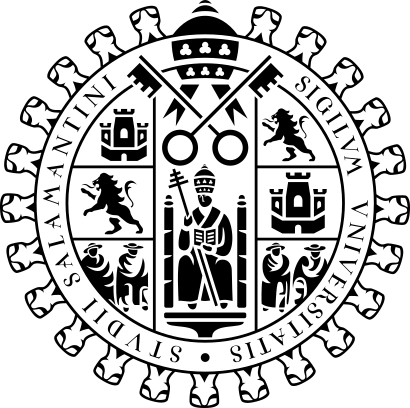
\includegraphics[width=2.5cm]{logo.png}}

\mode<article>{\lecturenumber{1}}

\begin{document}

\maketitle

\mode*  % ignore text outside frame in presentation mode

This is your lecture abstract. It should contain a short description of the lecture contents, what its goals are, and preferably not exceed a few dozen words.\marginnote{Do not forget to use margin notes to add more context to your material.}

\section{The largest prime number}

\begin{frame}
  \begin{theorem}
    There is no largest prime number.
  \end{theorem}%
  \pause
  \mode<article>{The proof uses reductio ad absurdum. Although this comment is inside a \texttt{beamer} frame, it only appears in the handout.}
  \begin{block}{Proof}
    \begin{enumerate}
      \item<alert@2> Suppose $p$ were the largest prime number.
      \item<alert@3> Let $\Pi$ be the product of the first $p$ primes.
      \item<alert@4> Then $\Pi + 1$ is not divisible by any prime.
      \item<alert@5> Therefore, $\Pi + 1$ is also a prime. \qedhere
    \end{enumerate}
  \end{block}
\end{frame}

You should restrain references to the bibliography outside frame environments, e.g.~\citet{newton1687} states that ``when arithmetical addition has been defined [it follows that] 1 + 1 = 2.''\cite{newton1687}

\section{The most beautiful equation}

\begin{frame}{Euler's identity}
  \begin{equation}
    e^{i\pi} + 1 = 0
  \end{equation}
\end{frame}

\begin{frame}<beamer>[standout]
  Thank you.
\end{frame}

\bibliographystyle{plainnat}
\bibliography{references}

\end{document}

